% \documentclass[notes]{beamer}       % print frame + notes
\documentclass{beamer}   % only notes
%\documentclass{beamer}              % only frames
\usepackage{LlabsTheme}

\usepackage[utf8]{inputenc}
\usepackage[T1]{fontenc}
\usepackage[german, english]{babel}
\usepackage{amsmath,amssymb,amsthm}
\usepackage{makeidx}
\usepackage{graphicx}
\usepackage{xspace}
\usepackage{url}
\usepackage{comment}
\usepackage{caption}

\usepackage{memhfixc}
\usepackage{hyphenat}
\usepackage{xcolor}

\usepackage[square,numbers]{natbib}
\bibliographystyle{abbrvnat}

\usepackage{afterpage}
\usepackage{refcount}
\usepackage{graphicx}

\usepackage{tikz}
\usetikzlibrary{decorations.text}
\usepackage{xcolor}
\usetikzlibrary{shapes}

\usepackage{url}
\usepackage{comment}
\usepackage{xspace}
\usepackage{siunitx}
\sisetup{locale = US}
\DeclareSIUnit{\mph}{mph}
\setlength\abovecaptionskip{2pt}

\captionsetup[figure]{font=tiny,labelfont=tiny}

%% to propeerly type 1st 2nd 3rd, usw
\newcommand\nd{\textsuperscript{nd}\xspace}
\newcommand\rd{\textsuperscript{rd}\xspace}
\newcommand\st{\textsuperscript{st}\xspace}

\newcommand\nth{\textsuperscript{th}\xspace} %\th is taken already


%\usepackage{algorithm}
%\usepackage{algpseudocode}

% \usepackage{algorithm2e}
% \usepackage{algorithmic}

%\usepackage{ngerman}      % language set to new-german
\usepackage[utf8]{inputenc}   % coding of german special characters
\usepackage[absolute,overlay]{textpos}
\usepackage{array}
\usepackage{setspace}
\newcommand{\RNum}[1]{\uppercase\expandafter{\romannumeral #1\relax}}
\newcommand{\argmin}{\operatornamewithlimits{argmin}}
\newcommand{\argmax}{\operatornamewithlimits{argmax}}
\newcommand{\meth}[1]{\texttt{\textbf{#1}}}

\newcommand{\csharp}{C\#\xspace}

\newcommand{\HL}[1]{{\color{primarycolor} #1}}

\usepackage{tikz}

\usepackage{hyperref}
\usepackage{graphicx}

\newcommand{\coo}{\ensuremath{\mathrm{CO_2}}}

\newcounter{thmcount}
\newtheoremstyle{break}% name
{}%         Space above, empty = `usual value'
{}%         Space below
{}% Body font
{}%         Indent amount (empty = no indent, \parindent = para indent)
{\bfseries}% Thm head font
{}%        Punctuation after thm head
{\newline}% Space after thm head: \newline = linebreak
{}%         Thm head spec

\usepackage{etoolbox}


\theoremstyle{break}
\newtheorem{exmp}{Example}[thmcount]
\newtheorem{obs}{Observation}[thmcount]
\newtheorem{cor}{Corollary}[thmcount]
\newtheorem{defn}{Definition}[thmcount]
\newtheorem{lem}{Lemma}[thmcount]

\usepackage{adjustbox}

\newcommand{\outgoing}{\emph{outgoing}\xspace}
\newcommand{\return}{\emph{return}\xspace}

\newcommand{\punctual}{\emph{punctual}\xspace}
\newcommand{\tardy}{\emph{tardy}\xspace}

\renewcommand*{\thefootnote}{\fnsymbol{footnote}}



\title[Oversize and heavyweight
cargo transportation considering bridge carrying capacity]{
\large
Optimal route selection for oversize and heavyweight
cargo transportation considering bridge carrying capacity
}

\author[Christian Wankm\"uller]{\small
Christian Wankm\"uller  \inst{1}
\and
Andreas Felsberger \inst{1}
\and
Christian Truden \inst{2}
}

\institute[LLabs]{\footnotesize
\inst{1} Department of Operations Management and Logistics, Alpen-Adria-Universit\"at Klagenfurt,
Klagenfurt, Austria
\inst{2} Lakeside Labs GmbH, Klagenfurt, Austria
}

\date{\footnotesize
31\st European Conference on Operational Research,\\
University of West Attica, Athens, Greece,\\
July 11-16, 2021
}





%Customized settings to define the style of the presentation

%%%%COLORS %%%%
%defines the used color scheme
\colorsAAU

%\titlelogoAAU  %%AAU logo on title frame
% \titlelogoLLabsLUC  %%LLAbs and LUC logo on title frame
% \titlelogoLLabsEFRE
\titlelogoAAULLabsSweet

%%%%LOGOS ON FRAMES %%%
%defines which logos are displayed on the frame, if you want to change the logos
%for certain frames, just apply the command before the \begin{frame} command
%all following frames will have the defines appearance
% \logoAAU
% \logoLlabsLUC
\logoAAULlabs
%\logoNONE

%%%HEADLINE
\headlineLEFT  %aligns the section overview in the headline LEFT
%\headlineCENTER %spreads the  section overview in the headline evenly


%%%FOOTLINE
%Define the appearance of the footline
%\footlineNUMBER  % show number of current slide
\footlineNUMBERTOTAL  % also shows the total number of slides
%\footlineNONUMBER  %no number displays

%%%%AVAILABLE COLORS%%%
%the following colors are predefined for use with the \color{col} command
%-   primarycolor
%-  secondarycolor

\begin{document}


\begin{frame}[plain]{\titlepage}\end{frame}
  %
  %
  %
  %
  %
  %   \section{Introduction}
  %
  %
  \begin{frame}
    \frametitle{Intro}
    \begin{itemize}
      \item \citet{Palsaitis.2012}
      \item \cite{Palsaitis.2012}

    \end{itemize}
  \end{frame}

  %
  \begin{frame}

    \begin{figure}[!ht]
      \centering
      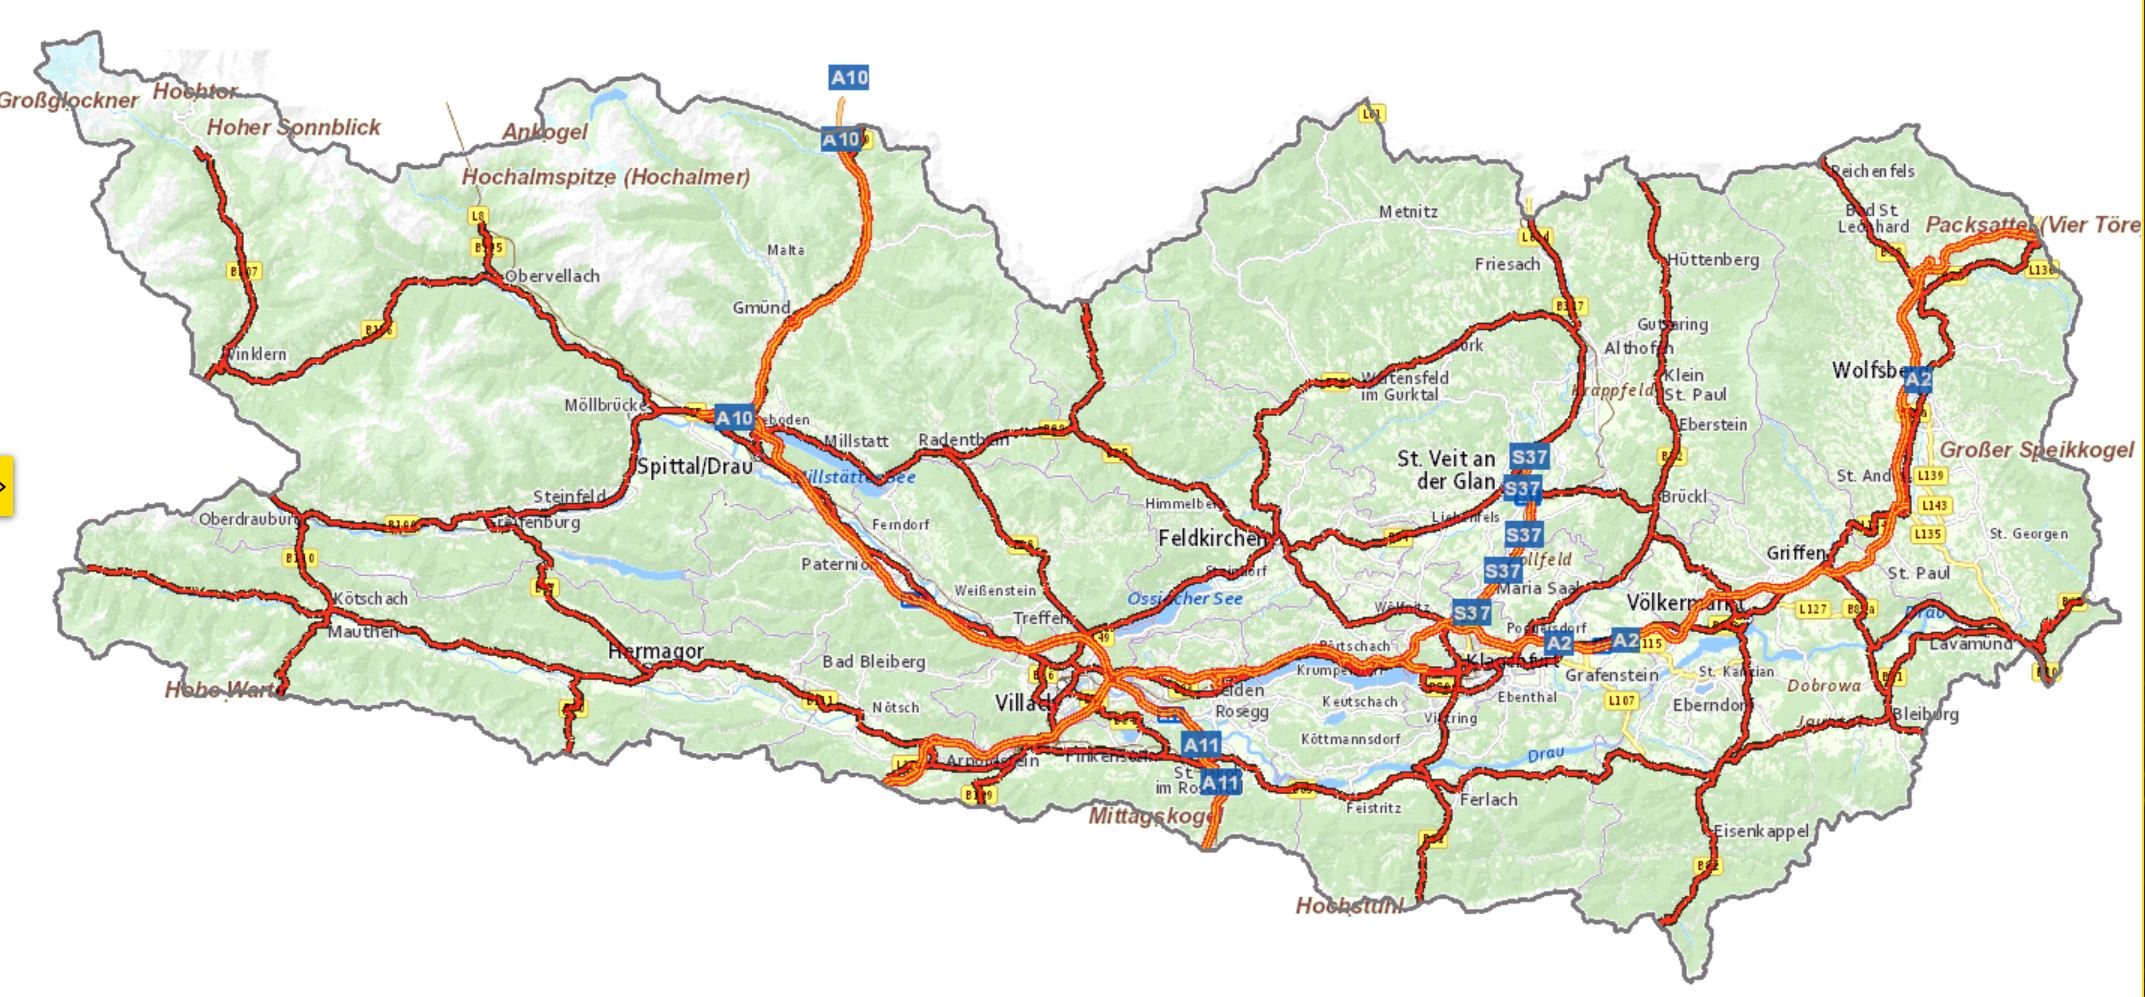
\includegraphics[width=1.0\textwidth]{../manuscript/figures/map.jpg}
      \caption{Overview of the higher level road network in Carinthia.}
      \label{fig:higher level}
    \end{figure}
  \end{frame}

  %
  %
  % A simple toy example, see Figure \ref{fig_toy_example_1}, shall illustrate these definitions.



  \begin{frame}
    \frametitle{Mathematical Model \RNum{1}}
    \begin{itemize}

      \item Classically,  the considered network $\mathcal{N}=(\mathcal{V},\mathcal{E})$ consists of
      \begin{itemize}
        \item \emph{Nodes} (vertices) $\mathcal{V}=\{1,\ldots, n\}$, which represent the intersections of road
        well as the start (end) points of the roads, and

        \item \emph{Links} (edges) $\mathcal{E} \subseteq \mathcal{L} \times \mathcal{L}$,
        correspond to the roads (road segements) connecting the vertices.
      \end{itemize}

      \item  Road links $e \in \mathcal{E}$ have a length $\ell(e)\in \mathbb{R}^{+}$ representing their road length.
      Further, they have a weights $c(e) \in C$ giving their \emph{classification} according to {\color{red} ??}.

      \item
      % Bridges have \emph{weight limits} (measured in metric tons) which are determined by civil engineers.
      Each road link $e \in \mathcal{E}$ contains a nonnegative number of bridges, where each has a weight limit.
      For each link $e$, we set a \emph{weight limit} $w(e) \in \mathbb{R}^{+}$ which is the
      minimum over all bridges on this link and the \emph{number of bridges} $b(e) \in \mathbb{N}^{0}$.

      \item Also  nodes $v \in \mathcal{V}$ can have weight limits.
    \end{itemize}

  \end{frame}



  \begin{frame}
    \frametitle{Mathematical Model \RNum{2}}

    \begin{itemize}
      \item
      A \emph{transport request} $r=(o,d,w) \in \mathcal{V} \times \mathcal{V} \times \mathbb{R}^{+}$
      has an \emph{origin} $s$, a \emph{destination} $t$, a \emph{total weight} $w$.

      \item A transport $r$ can only pass through nodes $v \in \mathcal{V}$ with
      $w(r) \leq w(v)$ and traverse road links $e \in \mathcal{E}$ for which $w(r) \leq w(e)$ holds.

      \item We define the sub-network $\mathcal{N}_{\omega}$ that contains only the vertices and edges from $\mathcal{N}$ that have a weight limit larger than $\omega \in \mathbb{R}^{+}$.

      \item We set $\mathcal{N}=\mathcal{N}_{\omega=w(r)}$.
    \end{itemize}

  \end{frame}



  \begin{frame}
    \frametitle{Mathematical Model \RNum{3}}
    \begin{align}
      \min \quad &\sum_{(i,j)\in \mathcal{E}}  c_{ij} x_{ij} \label{obj} \\
      \text{s.t.}\quad &
      \sum_{(i,j)\in \delta^{+} (i)} x_{ji} - \sum_{(i,j)\in \delta^{-}(i)} x_{ij} =
      \begin{cases}
        1 \quad& \text{if}~ i=s, \\
        -1 \quad& \text{if}~ i=t \\
        0 \quad&\text{else}
      \end{cases}
      \qquad \forall i \in \mathcal{E}
      \\
      &  \sum_{(i,j)\in \delta^{+} (i)} x_{ij}   x_ {ij} \leq 1     \qquad \forall i \in \mathcal{E}\\
      &  x_{ij} \in \{0,1\}   \qquad \forall (i,j) \in \mathcal{V}
    \end{align}
  \end{frame}


  \begin{frame}
    \frametitle{Objectives}
    We consider three different objectives, i.e., different assignment of $c_{ij}$.
    \begin{enumerate}
      \item \emph{Classic shortest path}, where $c_{ij}=\ell_{ij}$. \label{obj_short}
      \item \emph{Minimal number of surpassed briges}, where  $c_{ij}=b_{ij}$.  \label{obj_minBridge}
      \item \emph{Prefer high level roads}, where we assign an exponential weighting to the road classes (in ascending order of preference) $C$, $c_0=2^0,c_1=2^1, \ldots$.  \label{obj_highLevelRoad}
    \end{enumerate}
  \end{frame}
  \begin{frame}

    \begin{figure}[!ht]
      \centering
      \scalebox{0.7}{
      % !TeX root =../main.tex
% !TeX spellcheck = en_US

% https://tex.stackexchange.com/questions/64252/tikz-midway-label-on-a-bended-line
% https://texample.net/tikz/examples/p2p-topology/

\begin{tikzpicture}[auto, thick]

  % Define Colors
  \definecolor{pinegreen}{cmyk}{0.92,0,0.59,0.25}
  \definecolor{royalblue}{cmyk}{1,0.50,0,0}
  \definecolor{lavander}{cmyk}{0,0.48,0,0}
  \definecolor{violet}{cmyk}{0.79,0.88,0,0}
  \definecolor{red}{cmyk}{0,0.95,0.90,0}
  \definecolor{yellow}{cmyk}{0,0.25,1,0}

  % Node styles
  \tikzstyle{cblue}=[circle, draw, thin,fill=cyan!20, scale=0.8]
  \tikzstyle{qgre}=[rectangle, draw, thin,fill=green!20, scale=0.8]

  \tikzstyle{A_path}=[ultra thick, red, opacity=0.8, font=\small]
  \tikzstyle{S_path}=[ultra thick, yellow, opacity=0.8, font=\small]
  \tikzstyle{B_path}=[ultra thick, royalblue, opacity=0.8, font=\small]
  \tikzstyle{L_path}=[ultra thick, pinegreen, opacity=0.8, font=\small]


  % Nodes
  % \node[cblue] (n_1_1) at (0,0) {1};
  % \node[cblue] (n_2_1) at (4,0) {2};
  \node[cblue] (n_6) at (8,0) {6};

  % \node[cblue] (n_1_2) at (0,4) {4};
  \node[cblue] (n_4) at (4,4) {4};
  \node[cblue] (n_5) at (8,4) {5};

  \node[cblue] (n_1) at (0,8) {1};
  \node[cblue] (n_2) at (4,8) {2};
  \node[cblue] (n_3) at (8,8) {3};




  %  A links

  \draw[A_path,postaction={decorate,decoration={text along path,text align=center,text={$d=3, ~w=10$},raise=-10pt}}](n_4)--  (n_5)  node [midway, above, sloped] {$[10t]$};
  \draw[A_path,postaction={decorate,decoration={text along path,text align=center,text={$d=3.7, ~w=10$},raise=-10pt}}] (n_6) to[bend left]   node [midway, above, sloped]  {$[10t]$} (n_5)  ;
  \draw[A_path, postaction={decorate,decoration={text along path,text align=center,text={$d=4, ~w=10$},raise=-10pt}}] (n_1) -- (n_4)  node [midway, above, sloped]  {$[10t]~[10t]$};


  % S links
  \draw[S_path, postaction={decorate,decoration={text along path,text align=center,text={$d=8, ~w=10$},raise=-10pt}}] (n_4) to node [midway, above, sloped] {$[10t]$} (n_6);

  %  L lines
  \draw[L_path, postaction={decorate,decoration={text along path,text align=center,text={$d=4, ~w=10$},raise=-10pt}}] (n_1) --  (n_2)  node [midway, above, sloped] (TextNode) {$[10t]$};

  \draw[L_path, postaction={decorate,decoration={text along path,text align=center,text={$d=5$},raise=-10pt}}] (n_2)--  (n_3)  node [midway, above, sloped] (TextNode) {};
  % \draw[L_path] (n_3) to[out=-20,in=-20]  (n_5)  node [midway, above, sloped] (TextNode) {$l=3, b=2$};
  \draw[L_path,postaction={decorate,decoration={text along path,text align=center,text={$d=3, ~w=10$},raise=-10pt}}] (n_3) to[bend left] node [midway, above, sloped]   {$[10t]$}    (n_5);

  \draw[L_path, postaction={decorate,decoration={text along path,text align=center,text={$d=4.5$},raise=-10pt}}] (n_5) to[bend left]  node [midway, above, sloped] {} (n_6);

  % B links
  % \draw[B_path] (n_6) to node [midway, above, sloped] {$7; 2$} (n_2_1);


  % Legends
  % \node[A_path, anchor=west] at (-3,8){\textsc{A:} $w=2^0$};
  % \node[S_path,anchor=west] at (-3, 7.5){\textsc{S:} $w=2^1$};
  % \node[L_path,anchor=west] at (-3, 7){\textsc{L:} $w=2^2$};
  % \node[B_path,anchor=west] at (-3, 6.5){\textsc{B:} $w=2^3$};

  \node[ anchor=west] at (0,2){Levels: {\color{red}\textsc{A}}, {\color{yellow}\textsc{S}},  {\color{royalblue}\textsc{B}},  {\color{pinegreen}\textsc{L}}  } ;


\end{tikzpicture}

      }
      % \caption{Toy Example 1.}
      % \label{fig_toy_example_1}
    \end{figure}
  \end{frame}


  %     \frametitle{Motivation - Passenger Transportation in Rural Areas}
  %
  %     \begin{itemize}
  %       \item Transportation demand arises from the need to reach urban centers (work, school, etc.).
  %       \item Demand peaks around particular times due to low population density.
  %       \item Lack of transport provision for the first/last mile to/from public transport system corridors (timetabled services).
  %       \item Need for sustainable and reliable form of rural passenger mobility.
  %       \item Individual car use is (often) the only means of transportation.
  %       \item Major source of \coo-emissions (besides industry).
  %     \end{itemize}
  %   \end{frame}
  %
  %
  %   \begin{frame}
  %     \frametitle{Micro-Transit Systems}
  %     \begin{itemize}
  %       \item Demand-responsive ride-sharing options that are flexible in their service provision.
  %       \item Service provider's perspective
  %       \begin{itemize}
  %         \item \HL{Usage behavior} of passengers that use the system.
  %         \item \HL{Service provision}, service may vary in terms of modality, purpose, flexibility.
  %       \end{itemize}
  %       \item Customers may request transports
  %       \begin{itemize}
  %         \item \HL{Pre-booked}, well ahead of journey start time.
  %         \item \HL{Ad-hoc}, close to actual required travel time.
  %       \end{itemize}
  %       \item A successful service must find a balance between
  %       \begin{itemize}
  %         \item Convenience: all transport requests (including delayed) are serviced.
  %         \item Reliability: destinations are reached in time.
  %       \end{itemize}
  %
  %     \end{itemize}
  %   \end{frame}
  %
  %
  %
  %
  %   \section{Approach}
  %
  %
  %
  %
  %   \begin{frame}
  %     \frametitle{Transport Demand}
  %     \begin{itemize}
  %       \item \HL{Characteristics of a Transport Request}
  %       \begin{itemize}
  %         \item \textit{Origin / Destination}.
  %         \item \textit{Arrival Time Window} for transferring to time-tabled services.
  %         \item \textit{Pick-Up Time} at which passenger must be ready at location (given by Optimization).
  %       \end{itemize}
  %       \item
  %       \HL{Transport Request Chain}
  %       \begin{itemize}
  %         \item Several transport requests, which together define a sequence of journey legs, are scheduled in an "all or nothing" fashion by a provider.
  %         \item A transport chain is regarded as ``broken'' when a passenger misses the pick-up time, and ceases to be serviced.
  %       \end{itemize}
  %
  %       \item Commuter requests
  %       \begin{itemize}
  %         \item \textit{Outgoing request}: towards train/bus stations in the morning.
  %         \item \textit{Return request}: in the evening.
  %       \end{itemize}
  %
  %     \end{itemize}
  %   \end{frame}
  %
  %
  %
  %   \begin{frame}
  %     \frametitle{Challenges for the Service Provider}
  %
  %     \begin{itemize}
  %       \item How does the \HL{punctuality} of the passengers affect service provision?
  %       \vspace*{0.4cm}
  %       \item Should drivers wait for late passengers? For how long?
  %       \vspace*{0.4cm}
  %       \item How can the service provider identify a reasonable policy for how to deal with late (unpunctual) passengers?
  %     \end{itemize}
  %   \end{frame}
  %
  %
  %   \begin{frame}
  %     \frametitle{Overall Approach}
  %     \vspace*{-1cm}
  %     \begin{adjustbox}{max totalsize={.9\textwidth}{.7\textheight},center}
  %       \begin{tikzpicture}
  \node (opt) at (0,0) [draw,thick,minimum height=0.8cm] {\bf Optimization};
  \node (sim) at (5,0) [draw,thick,minimum height=0.8cm] {\bf Simulation};
  \node (pop) at (-2.5, 1.2)  {\begin{tabular}{c}Synthetic Population \\ (OD-Pairs) \end{tabular} };
  \node (res) at (7, 1.2)  {\begin{tabular}{c}Experimental \\ Results \end{tabular} };
  \draw[->,line width=0.8mm] (opt) -- (sim)  node [midway,align=center]{\begin{tabular}{c}Transport \\ Schedules \end{tabular}}  ;
  \draw[->,line width=0.8mm]  (pop) -- (-2.5,0)  -- (opt);
  \draw[->,line width=0.8mm]  (sim) -- (7,0)  -- (res);
\end{tikzpicture}

  %     \end{adjustbox}
  %     \begin{enumerate}
  %       \item Create transport schedules using \textit{Large Neighborhood Search} [Ropke \& Pisinger 2006] for
  %       a multi-objective variant of the \textit{Dial-a-ride problem} (DARP).
  %       \item Use Agent-based Modeling (ABM) and Simulation to analyze the influence of external factors on the execution of transport schedules.
  %       \item Fine-tune parameters of service provision based on the simulation results.
  %     \end{enumerate}
  %   \end{frame}
  %
  %
  %   \begin{frame}
  %     \frametitle{Agent-based Model}
  %
  %     \begin{itemize}
  %       \item \HL{Cycle.} \textit{Event} (time) $\rightarrow$ \textit{Activity} (randomness) $\rightarrow$ \textit{Event}.
  %       \item \HL{Vehicle Agents}
  %       \begin{itemize}
  %         \item Encapsulate vehicles and assigned drivers.
  %         \item Mission: follow the transport schedule.
  %         \item Activities: (i) transfer between stops, (ii) arrive (leave) at (from) stop, (iii) wait for passengers, etc.
  %       \end{itemize}
  %       \item \HL{Passenger Agents}
  %       \begin{itemize}
  %       \item Mission: complete their trip plan (derived from vehicle schedules).
  %       \item Activities: (i) walk to location, (ii) arrive at location,
  %       (iii) (un)board vehicle, (iv) wait for vehicle, etc.
  %       \end{itemize}
  %       \item \HL{Stop Agents}
  %       \begin{itemize}
  %         \item Passive role, serve as ``interface'' between passengers and vehicles.
  %       \end{itemize}
  %     \end{itemize}
  %   \end{frame}
  %
  %
  %   \section{Analysis}
  %
  %   \begin{frame}
  %     \frametitle{Passenger Types}
  %
  %     \vspace*{-0.8cm}
  %     \begin{itemize}
  %       \item Two types of passengers
  %       \begin{itemize}
  %         \item \HL{Punctual}, show up at pick-up location mostly ahead of pick-up time.
  %         \item \HL{Tardy}, arrive closer to or even later than at the scheduled pick-up time.
  %       \end{itemize}
  %       \item Sources of randomness
  %       \begin{itemize}
  %         \item  Departure from home (or last destination) towards pick-up location (Normal Distribution).
  %         \item Walking time (Truncated Normal Distribution).
  %       \end{itemize}
  %       % \item Population types
  %       %   \begin{itemize}
  %       %     \item \si{80\,\percent} punctual passengers.
  %       %     \item \si{50\,\percent} punctual passengers.
  %       %     \item \si{20\,\percent} punctual passengers.
  %       %   \end{itemize}
  %     \end{itemize}
  %     \begin{figure}
  %       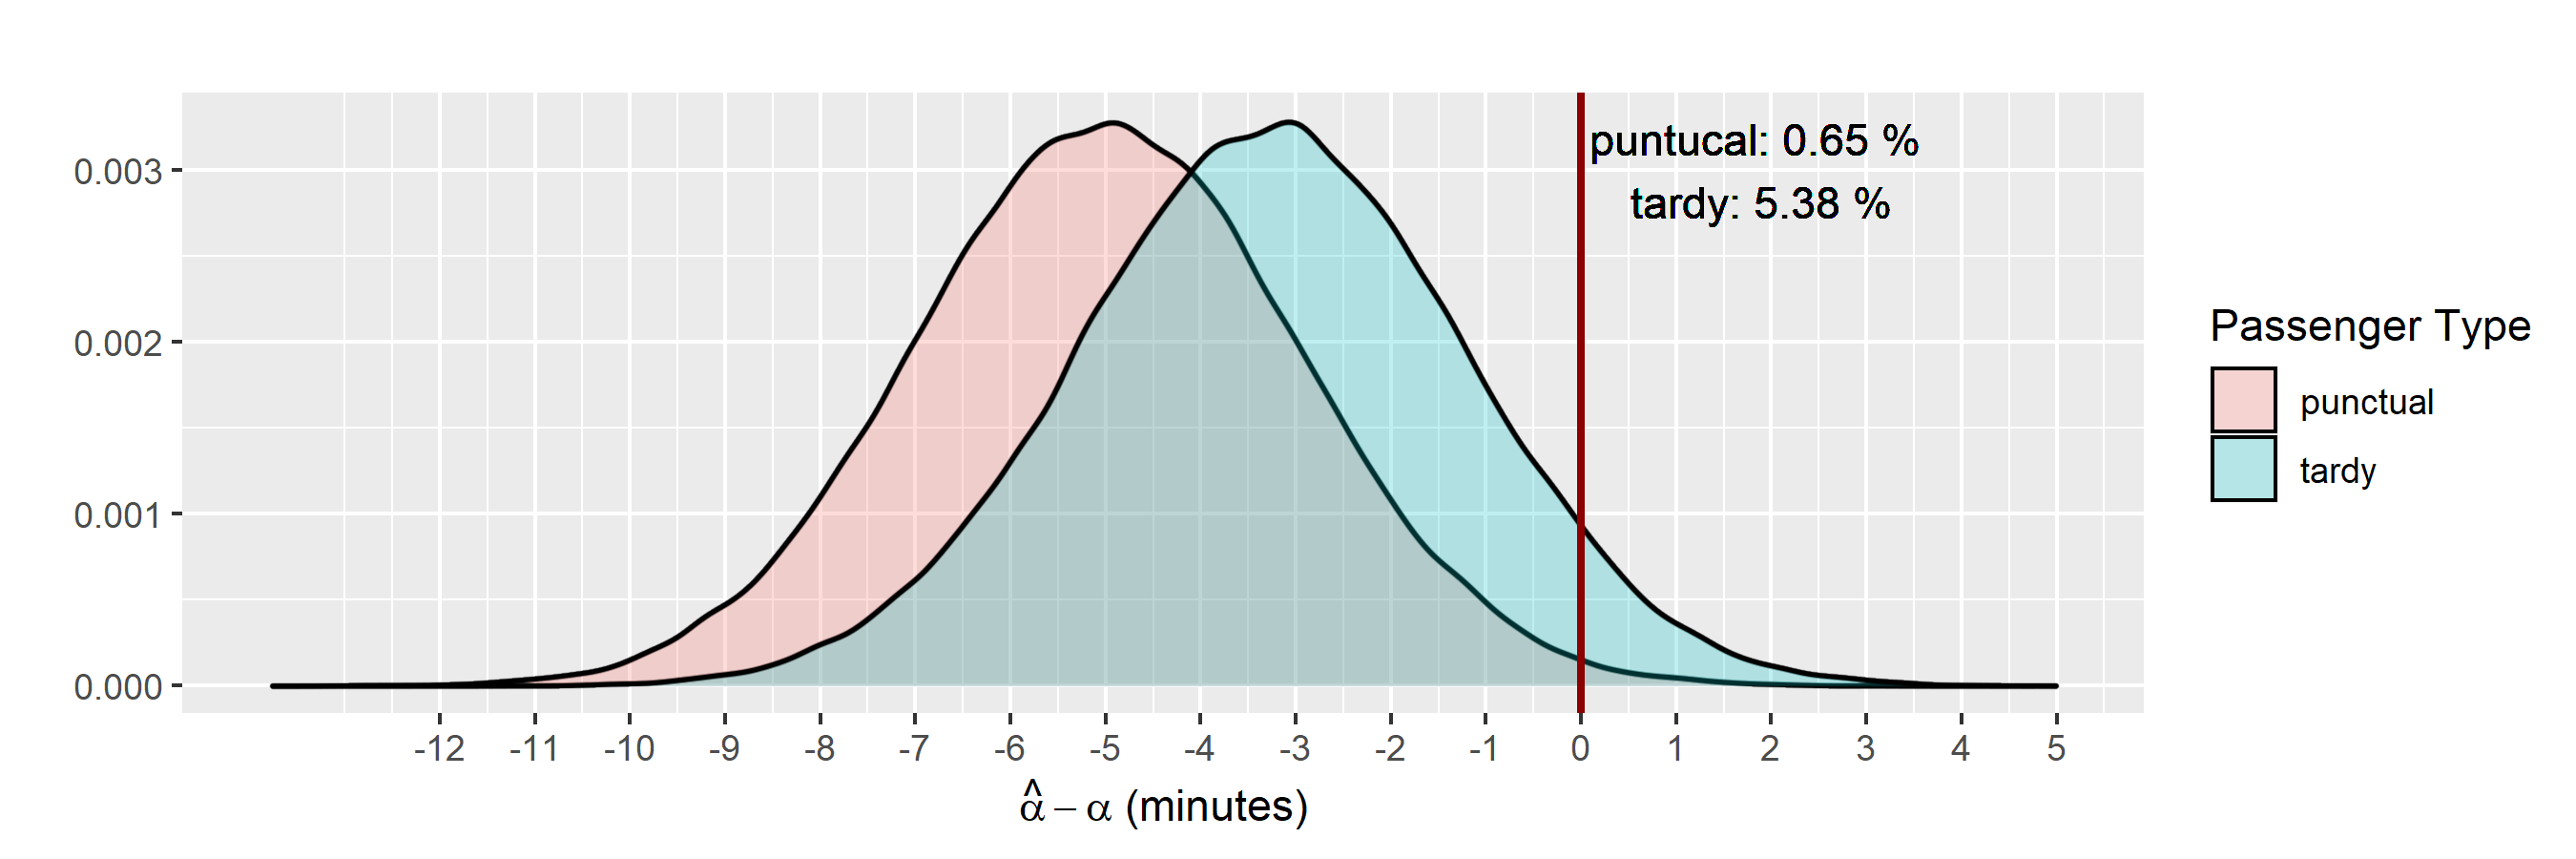
\includegraphics[width=0.9\textwidth]{./figures/passengerProfiles.png}
  %
  %     \end{figure}
  %   \end{frame}
  %
  %
  %   \begin{frame}
  %     \frametitle{Experimentation}
  % %Implementation of simulations in  \csharp.
  % We used the following setup for our simulation runs:
  %     \begin{itemize}
  %       \item \num{100} commuters, \num{10} vehicles.
  %       \vspace*{0.2cm}
  %       \item \num{10} samples, consider all vehicle transport schedules where all transport chains have been accepted.
  %       \vspace*{0.2cm}
  %
  %       \item \num{100} simulation runs each ($\sim$ \num{5}\,seconds).
  %       \vspace*{0.2cm}
  %
  %       \item Varying waiting time for late passengers $\omega$.
  %     \end{itemize}
  %   \end{frame}
  %
  %
  %   \begin{frame}
  %     \frametitle{Results: $\omega=0$ (no waiting for late passengers)  \RNum{1}}
  %     \vspace*{-1cm}
  %     \begin{figure}
  %       \includegraphics[width=0.9\textwidth]{./figures/both.pdf}
  %       % \caption{}
  %       % \label{}
  %     \end{figure}
  %     \vspace*{-0.2cm}
  %         \begin{itemize}
  %     \item  More punctual passengers $\rightarrow$ earlier arrival.
  %     \item  Good portion of the passengers arrive within the arrival time window.
  %     \item  Arrival at destination is rarely more than $5$\,min later than planned arrival time window (given experimental population).
  %     \end{itemize}
  %   \end{frame}
  %
  %
  %   \begin{frame}
  %     \frametitle{Results: $\omega=0$ (no waiting for late passengers) \RNum{2}}
  %     \footnotesize
  %     \centering
  %     % !TeX root = main.tex
% !TeX spellcheck = en_US

\begin{tabular}{
   S[table-format=2.0, table-column-width=1.5cm]
    |
S[table-format=2.2, table-column-width=1.5cm] 
 rrrrr
  }
  \hline
 {\punctual}    &    {$\ell >0$}    &  {$q_{25}$} &    {$q_{50}$}  &  {$q_{75}$} & {$q_{95}$}    &  {$q_{99}$}
 \\
   {(\%)}   &      {(\%)}    &  {(mm.ss)} &    {(mm.ss)}  &   {(mm.ss)} &  {(mm.ss)}    &   {(mm.ss)}
   \\
  \hline
 80  & 10.80466 & -13.53& -7.58 & -2.45 & 1.27 & 4.07  \\
  50  &  12.11865   & -13.20 & -7.31  & -2.15 & 1.34 & 4.10  \\
  20   & 13.26574 & -12.52 & -7.10  & -1.51 & 1.40 & 4.14  \\
  \hline
\end{tabular}
 % \maxf{-0.001589677}




  %     \vspace*{1cm}
  %     % !TeX root = main.tex
% !TeX spellcheck = en_US

\begin{tabular}{
   S[table-format=2.0, table-column-width=1.5cm]|
  S[table-format=2.2, table-column-width=2cm]
  S[table-format=2.2, table-column-width=2cm]
  S[table-format=2.2, table-column-width=2cm]
  }
  \hline
  {\punctual}     &    {aborted \outgoing}    &    {aborted \return}   & {both completed}\\
  {(\%)} &       {(\%)}       &  {(\%)}    &  {(\%)}  \\

  \hline
  80        & 3.56    & 1.82 &  94.6   \\
  50       & 4.74     &  3.06 & 92.2  \\
  20        & 5.83     & 4.22 &  90.0   \\
  \hline
\end{tabular}
 % \maxf{-0.001589677}
% 80        & 1339991  & 3.56    & 1.82 &  94.6   \\
 % 50        & 1339981 & 4.74     &  3.06 & 92.2  \\
 % 20        & 1339977 & 5.83     & 4.22 &  90.0   \\

  %   \end{frame}
  %
  %
  %   \begin{frame}
  %     \frametitle{Results: $\omega=0,\ldots,10$\,min   \RNum{1}}
  %     \vspace*{-0.4cm}
  %
  %     \begin{figure}
  %       \includegraphics[width=1\textwidth]{./figures/aborted_differentWaitTimes.pdf}
  %       % \caption{}
  %       % \label{}
  %     \end{figure}
  %       \begin{itemize}
  %     \item  Percentage of aborted requests goes down when introducing a waiting policy.
  %     \item  Extensive waiting time $\omega$ leads to raising numbers again.
  %     \item  Effect of  \HL{punctuality} is consistent over all experiments.
  %     \end{itemize}
  %   \end{frame}
  %
  %
  %   \begin{frame}
  %  %   \frametitle{Results: $\omega=0,\ldots,10$\,min   \RNum{2}}
  % %\vspace*{-1.5cm}
  % \vspace*{0.2cm}
  %     \begin{figure}
  %       \includegraphics[width=0.9\textwidth]{./figures/quantiles_h5.pdf}
  %       % \caption{}
  %       % \labelq{}
  %     \end{figure}
  %         \begin{itemize}
  %     \item  Quantile values move (increase) with increasing waiting time $\omega$.
  %     \item  This effect is rather weak.  Values do not increase by more than $1$\,min ($99\,\%$ quantile).
  %     \end{itemize}
  %   \end{frame}
  %
  %
  %   \section{Conclusion}
  %   \begin{frame}
  %     % \frametitle{Conclusion}
  %     \vspace*{1cm}
  %     \HL{Conclusion}
  %     \begin{itemize}
  %       \item Analysis of real-world performance of transport schedules for
  %       \textit{dial-a-ride} problem.
  %       \item Agent-based modeling and simulation to execute the schedules under the influence
  %       of disturbances.
  %
  %       \item Punctuality of passengers affects service provision.
  %       \item Introducing a waiting policy can improve service.
  %       \item Service providers can use the presented approach to fine-tune their policies.
  %     \end{itemize}
  %     \HL{Future Work}
  %
  %     \begin{itemize}
  %       \item Explore relationship between late arrival of \HL{vehicles} and aborted requests
  %       in more detail.
  %       \item Apply approach to urban settings.
  %     \end{itemize}
  %   \end{frame}



  %%%%%%%%%%%%%%%%%%%%%%%%%%%%%%%%%%%%%%%%%%%%%%%%%%%%%%%%%%%%%%%%



  %%%REFERENCES
  %if no references used, comment this section

  \appendix
  \begin{frame}[allowframebreaks]
    \frametitle{References}
    \vspace*{-1cm}
    \tiny
    \bibliographystyle{abbrvnat}
    \bibliography{../manuscript/bibliography}
  \end{frame}


  \begin{frame}[plain]{\titlepage}\end{frame}
    \end{document}
